\section{Einleitung}
\label{section:Einleitung}

Der Transport von Daten, insbesondere sensibler Daten über das Internet, ist Teil der heutigen Web-Anwendungen, wie \textcite[1]{kirda2009} in ihrer Studie erwähnen. Typischerweise interagieren Web-Anwendungen mit Backend-Datenbanken, um Daten dort abzufragen und zu empfangen, um diese dann als dynamisch generierten Inhalt an den Benutzer der Anwendung auszuliefern, so \textcite[1]{su2006}. Laut \textcite[1857]{chaudhari2014} handelt es sich immer um eine verteilte Anwendung auf Server und Client.

Eine sichere Web-Anwendung sollte Sicherheitseigenschaften, wie logische Korrekheit, Eingabe Validierung und Sanitazition vorweisen können.
Die logische Korrektheit bedeutet, dass die Anwendungslogik genau so korrigiert werden sollte, wie es von den Entwicklern beabsichtigt ist.
Die Gültigkeit der Eingaben bezieht sich auf die Benutzereingaben, die vor der Verwendung  durch die Anwendung validiert wurden. Die Integrität des Zustands bedeutet, dass der Anwendungszustand nicht verändert werden sollte und die Fehlkonfiguration der Sicherheit sich auf die Konfigurationseinstellungen unter Verwendung sicherer Komponenten bezieht.\autocite[1857]{chaudhari2014}

Jede Web-Anwendung hat ihre eigene logische Richtigkeit gemäß deren eigener Business Logik. Im globalen Sinne bedeutet dies, dass die Nutzer nur auf die zur Verfügung gestellten Informationen und Abläufe der Anwendung zugreifen können, sowie, dass diese dem beabsichtigten Abflauf der Anwendung folgen.\autocite[1857]{chaudhari2014}

Die Eingabe Validierung stellt sicher, dass Eingaben vom Nutzer zuerst überprüft und als gut bestätigt werden, bevor diese von der Web-Anwendung verwendet werden. Diese Validierung sollte auf der Client Seite, sprich dem Web-Browser geschehen, damit man der Server Seite versichern kann, dass die verarbeitenden Werte seriös und sinnvol sind.\autocite[1857]{chaudhari2014}


% Einleitungstext......
% wird nach Vollendung aller anderen Texte geschrieben, sowie Abstract und Kurzzusammenfassung.

\section{Hintergrund und Angriffsarten von XSS}
\label{section:Hintergrund}

In der heutigen Zeit nutzen die meisten Webseiten die Funktionalität von JavaScript im Web-Browser als deren großen Vorteil, doch trotz Einhaltung der same origin policy kann immer noch die Sicherheit des Systems verletzt werden. Dies geschieht, wenn beispielsweise ein Nutzer dazu gebracht wird, sich schadhaften JavaScript Code, welcher zuvor von einem Angreifer erstellt worden ist, auf sein System herunterzuladen. Diese im wahrsten Sinne des Wortes technische Ausbeutung nennt man eine cross-site scripting (XSS) Attake.\autocite[2]{kirda2009}


\textcite[2]{hydara2015a} melden, dass diese Sicherheitslücken erstmals in den 1990er, in den frühen Anfängen des World Wide Web, aufgetreten sind. Cross-Site-Scripting(XSS) gehört zu den ernstzunehmendsten Schwächen wenn es um Web-Anwendungen geht. Zu Schaden kommen dabei nicht nur der Source Code oder die Datenbank der Web Anwendung, sondern auch der Nutzer.

Laut OWASP \footnote{\url{https://www.owasp.org/index.php/Cross-site_Scripting_(XSS)}} gibt es drei Arten, wie XSS Attacken durchgeführt werden können.
\begin{itemize}
	\item reflected
	\item stored
	\item DOM-based
\end{itemize}
Diese drei Arten werden grundsätzlich in die zwei Kategorien reflected oder persistent und stored oder non-persistent unterteilt. Die dritte, viel weniger bekannte Art einer XSS Attacke wird DOM-based genannt.


XSS selbst, ist ein Angriff auf den Client-seitigen Web-Browser, welcher den tatsächlichen Schaden aber auf der Server-Seite verursacht. Für die Ausnutzung von XSS-Schwachstellen in den Web-Anwendungen fertigt ein Angreifer eine bösartige JavaScript Sprengladung an und injiziert diese dann in die Web-Anwendung. Dieses Skript wird so injiziert, dass es als gutartiger Bestandteil der Website erscheint, was dazu führt, dass das fremde Skript als vertraulich angesehen wird und in der originalen Domäne der Website ausgeführt wird.\autocite[5]{gupta2017}


Beide Arten von XSS Attacken, reflected und stored werden auf der Server-Seite ausgeführt. Dies passiert immer dann, wenn eine Anfrage an den infizierten Server geschickt wird. DOM-based XSS Attacken werden dahingegen auf der Client-Seite, also im Web-Browser ausgeführt. In allen Fällen sind Angreifer in der Lage sensible Daten von den Opfern zu stehlen.\autocite[2]{hydara2015a}

Der Ablauf um einen solchen Code in eine Anwendung injezieren zu können ist stets gleich, so \textcite{mahmoud2017}.
\begin{enumerate}
	\item Der Angreifer muss eine Schwachstelle in der Anwendung finden um seinen schadhaften Code in die Anwendung zu bringen und somit in weiterem Verlauf sensible Daten von seinem Opfer stehlen zu können.
	\item Das Opfer besucht die beschädigte Anwendung.
	\item Die Anwendung sendet eine Anfrage mit dem fehlerhaften Code im Body an einen Server.
	\item Wenn das Skript im Web-Browser des Opfers ausgeführt wird, kann der Angreifer diverse persönliche Informationen stehlen.
\end{enumerate}

\begin{figure*}[ht]
	\centering
	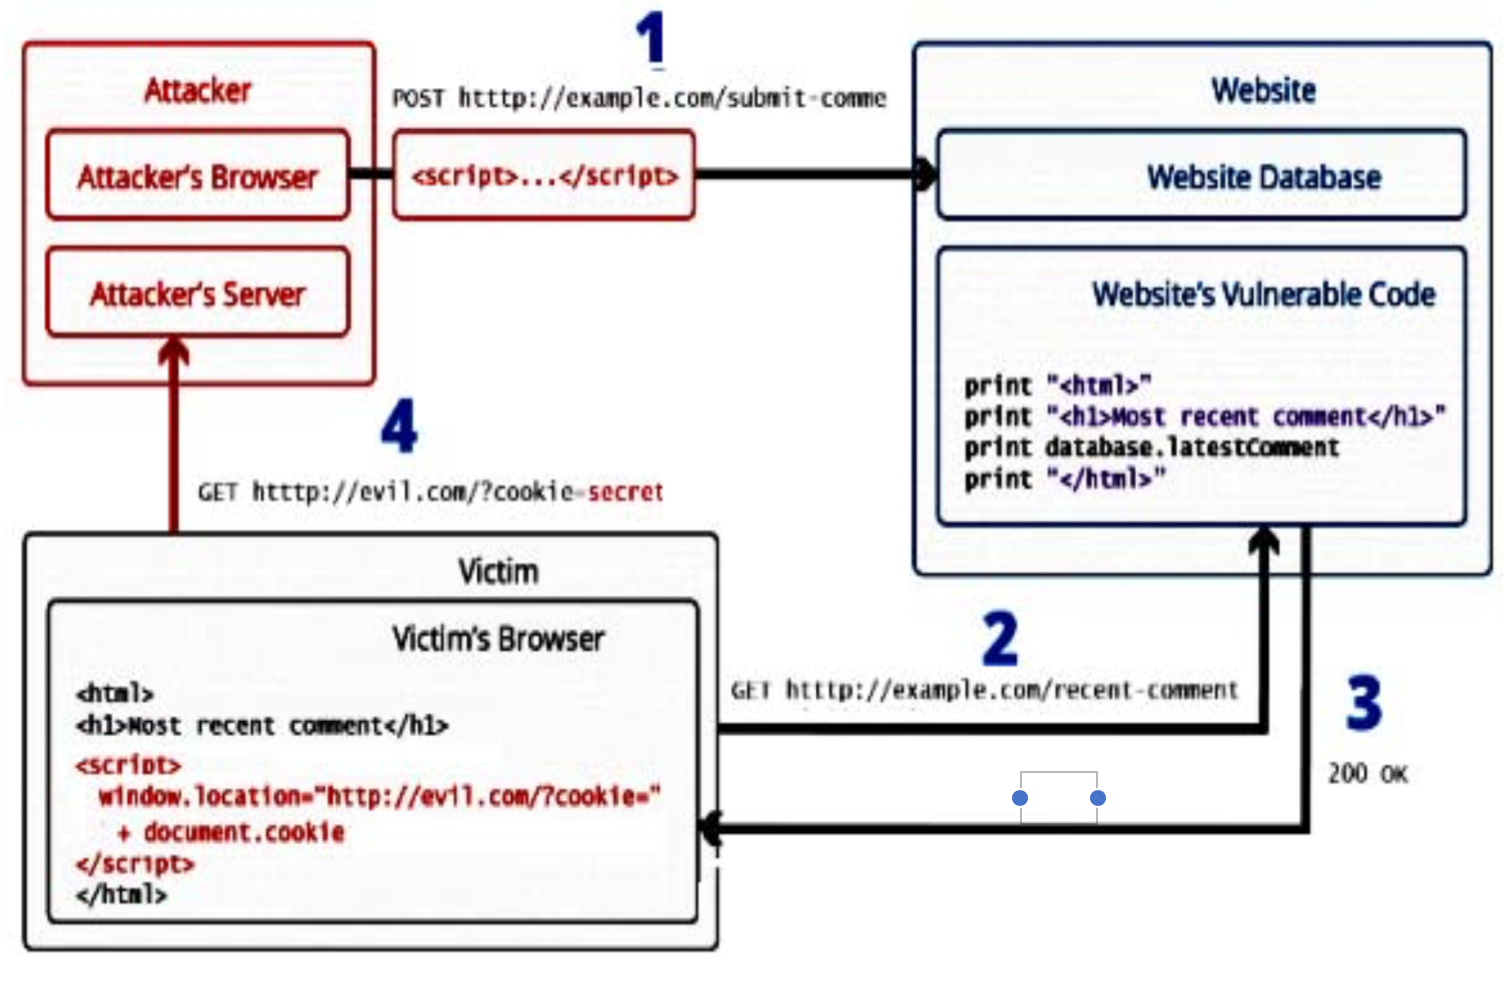
\includegraphics[width=0.8\linewidth]{images/XSS-attack-process.png}
	\caption{XSS Angriffsprozess\autocite[p]{mahmoud2017}}
\end{figure*}




% Ab hier genauere Info über Angriffsarten
\subsection{Stored oder Persistent Attacken}
\label{subsection:stored attacks}

Um eine stored XSS Attacke, oder auch persistente bzw. dauerhafte XSS Attacke erfolgreich ausführen zu können, muss der Täter Bob zuerst eine Schwachstelle in einer Web-Anwendung finden, um dort seinen schadhaften JavaScript Code auf den Server laden zu können.
Um solche Schwachstellen zu finden, probiert Bob HTML tags wie beispielsweise \verb+<h1>Hello World!</h1>+ in etlichen Eingabefeldern wie Kommentar-, oder Suchfeldern aus. Wird dieser tag vom Web-Browser als HTML tag interpretiert, weiß Bob, dass er auf dieser Seite sein Skript platzieren kann.
Hierzu fügt er anstatt eines h1 tags, einen script tag in das Kommentarfeld ein.
\begin{lstlisting}[
	label={},
	float=h,
	language=html,
	xleftmargin=0.5em,
	framexleftmargin=0.5em,
	tabsize=2,
	numbers=none
]
Best Product, read review here
<script src="http://evil.com/evil.js"> </script>
\end{lstlisting}

Durch diese Zeile JavaScript Code im Kommentarfeld wird nun jedes Mal, wenn diese Seite geladen wird, das Skript, welches auf evil.com gehostet wird, ausgeführt.

Diese Art von XSS Angriff kann eine große Menge an Opfer finden, denn verteilt man den Link von der angeblich sicheren Seite, gefährdet dies jeden Besucher, ganz egal wie Vorsichtig dieser sonst auch ist.

Aus der Sicht von Bob, ist es um einiges schwieriger eine dauerhafte XSS Attacke durchzuführen, weil er nicht nur eine Schwachstelle in der Web-Anwendung finden muss, sondern auch eine Web-Anwendung, welche einen großen Pool an Nutzern hat. Stimmen jedoch diese zwei Punkte überein, kann sehr großflächiger Schaden entstehen.

\footnote{\url{https://www.imperva.com/learn/application-security/cross-site-scripting-xss-attacks/}}


\subsection{Reflected oder Non-Persistent Attacken}
\label{subsection:reflective attacks}

Eine reflected XSS Attacke ist im Vergleich zu einer stored XSS Attacke in diesem Sinne anders, als dass sie von einer Web-Anwendung reflektiert wird, und nicht dauerhaft ist. Bei so einem Angriff wird der schadhafte JavaScript Code nur etwa durch einen Link ausgelöst.
Um dies zu erreichen wird meist ein Link zu einer Web-Anwendung mit Schwachstellen erstellt, in welcher der schadhafte JavaScript Code in einer E-Mail oder in einem HTML form Element eingebunden wird. Um solche Schwachstelle in einer Web-Anwendung zu finden, wird beispielsweise in einem Suchfeld
\begin{lstlisting}[
	label={},
	float=h,
	language=html,
	xleftmargin=0.5em,
	framexleftmargin=0.5em,
	tabsize=2,
	numbers=none
]
<scrip type="text/javascript">aler(XSS detected)</script>
\end{lstlisting}

ausgeführt und untersucht, ob dieser JavaScript Code vom Web-Browser als solcher interpretiert und ausgeführt wird, oder nicht.
Wird diese Popup ausgeführt, der Skripttext in der URL angezeigt oder wird im Web-Browser auf die Seite verwiesen und ein not found zurückgegeben, weiß der Angreifer, dass diese Seite anfällig ist.

Im nächsten Schritt erstellt er eine eigene URL und verpackt diese in einen Link welcher in einem Forum oder einem sozialen Netzwerk geteilt wird.
\begin{lstlisting}[
	label={},
	float=h,
	language=html,
	xleftmargin=0.5em,
	framexleftmargin=0.5em,
	tabsize=2,
	numbers=none
]
http://trusted.com?q=news<script%20src="http://evil.com/evil.js"
\end{lstlisting}

Obwohl die URL verdächtig ist, heißt es nicht, dass niemand diesen Link anklickt.
Darüber hinaus kann ein Angreifer auch eine URL-Adresse erstellen, die ein Benutzer nicht direkt interpretieren kann. Der Angreifer wird also die Kodierungsschemata ausführen, um die ASCII-Zeichen in das Hexadezimalformat zu konvertieren, wie im Skript S5 gezeigt. Nun kann das Opfer die URL nicht interpretieren, die im Hexadezimalformat erstellt wurde, und es ist wahrscheinlicher, dass der Angreifer diese URL besuchen kann.\autocite[125]{gupta2015a}

Wenn auch nur einer von tausenden Empfänger dieser E-Mail den Link klickt, ist Alice, die Täterin erfolgreich. Bob wird auf die Forumseite weitergeleitet, wo dar schadhafte JavaScript Code dann vom Web-Browser ausgeführt wird.

\footnote{\url{https://www.imperva.com/learn/application-security/reflected-xss-attacks/}}

\subsection{DOM-basierte Attacken}
\label{subsection:DOM-based Attacks}

DOM XSS steht für Document Object Model basiertes cross-site scripting. Diese Art von XSS ist dann möglich, wenn die Web-Anwendung Daten, welche nicht ordnugngsgemäß behandelt werden, in das DOM schreibt.
Der Angreifer Bob kann die Daten der Web-Anwendung oder der Webseite mittels schadhaftem JavaScript Code manipulieren.

Ein typisches Beispiel einer solchen Attacke, kann wie folgt aussehen.
Die Webseite \url{http://trusted.com/user.html} ist individuell vom Nutzernamen abhängig. Dieser ist kodiert in der URL und wird auf der Webseite direkt verwendet.

\begin{lstlisting}[
	label={},
	float=h,
	language=html,
	xleftmargin=1.5em,
	framexleftmargin=1.7em,
	numbersep=0.2em,
	caption={[XSS quelle] DOM-based XSS Example}
]
<!DOCTYPE html>
<html>
<head>
...
    <title>Greeting</title>
</head>
<body>
	Hello
	<script>
		let pos = document.URL.indexOf("name=");
		document.write(document.URL.substring(pos, document.URL.length));
	</script>
</body>
</html>
\end{lstlisting}

Ruft man die Seite \url{http://trusted.com/user.html?name=Max} auf, resultiert dies in einer angepassten Begrüßung für Max. Ersetzt man jedoch den name Parameter mit einem Skript-tag und ruft \url{http://trusted.com/user.html?name=<script>Evilfunction()</script>} auf, sendet der Web-Browswer eine HTTP Anfrage an \url{http://trusted.com} und bekommt eine statische HTML Seite zurück. Der Web-Browser baut das DOM auf und füllt die Eigenschaft \textbf{document.URL} mit der URL, welche das Skript enthält.
Der Web-Browser parsed die HTML Seite, bei document.URL angekommen, und führt das Skript aus und lädt dabei den schadhaften Code von der document.URL. Ist die Seite vollständig geladen, befindet sich der JavaScript Code vom Angreifer im DOM und wird durch den Interpreter im Web-Browser ausgeführt.

DOM-based XSS Attacken sind der Typ von XSS Angriffen, die im Document Object Model (DOM) einer HTMl Seite stattfinden, so dass der HTTP-Antwort-Code auf eine andere Art und Weise läuft. DOM XSS Angriffe können von einer Vielzahl von DOM Objekten durchgeführt werden. \autocite[763]{swaswatigoswami2017}

\begin{itemize}
	\item Username oder Passwort als Teil von location oder URL \newline In diesem Fall wird der Payload vom Server im Authentication Header vom Server empfangen.
	\item Ein Teil, wo sich der Queryteil in der URL befindet \newline In diesem Fall ist der Payload Teil der URL in der HTTP Anfrage
	\item Fragment eines Teils einer URL \newline Dieser Teil enthält im wesentlichen des Payload in der URL getrennt durch das ''\text{\#}'' Symbol. In diesem Fall wird der Payload nicht vom Server empfangen
	\item HTML DOM Referrer Objekt \newline Das Referrer Objekt ist \url{document.referrer} welches die URL des aktuell geladenen Dokuments represäntiert. In diesem Fall wird der Payload Teil im Referrer Header vom Server empfangen.
\end{itemize}


\section{Erkennunng}
\label{section:Detection}

Die Erkennung von Angriffen geht einher mit dessen Ausführung.
In früheren Umfragen haben \textcite[10]{gupta2014} Schritte zur Erkennung ob eine Webseite oder eine Web-Anwendung einer XSS Attacke gegenüber gefährdet ist oder nicht. Befolgt man die nun folgende Reihenfolge von Punkten, so kann man herausfinden ob seine Webseite anfällig ist für XSS Angriffe. Greifen Sie in der Entwicklung der Webseite oder Web-Anwendung immer wieder auf die Anwendung zu und suchen Sie speziell die Teile der Webseite auf, welche eine Eingabe vom Nutzer erfordern. Solche Kennzeichnungen findet man in Loginformularen, Suchfeldern, Kommentaren, etc. Im nächsten Schritt geben Sie einen beliebige Zeichenfolge ein und senden Sie diese mittels HTTP Anfrage an den Server. Interessant ist hier die Antwort des Servers. Vergleicht man die HTTP Anfrage und die HTTP Antwort, darf die eingegebene Zeichenkette nicht eins zu eins in der Antwort des Servers enthalten sein. Ist dies der Fall, dann handelt es sich um eine Schwachstelle gegenüber XSS in Ihrer Webseite.
Ist die Zeichenfolge jedoch nicht in der Antwort des Servers enthalten, testen Sie die nächste Bedingung. Hierfür geben Sie nun einen JavaScript Code, wie beispielsweise
\begin{lstlisting}[
	label={},
	float=h,
	language=html,
	xleftmargin=0.5em,
	framexleftmargin=0.5em,
	tabsize=2,
	numbers=none
]
<script>alert("XSS")<\script>
\end{lstlisting}
in das Eingabedeld ein und starten Sie erneut einen HTTP Anfrage. Sollte jetzt ein Pop-Up Fenster mit dem Text XSS Schwachstelle erscheinen, dann ist ihre Anwendung für XSS Attacken anfällig. Öffnet sich kein Pop-Up, bedeutet dies, dass Sie Ihre Webseite ordnugngsgemäß gegenüber von XSS Attacken geschützt haben.

Verschieden Erkennungsmethoden haben unterschiedliche Anaylsemechanismen. Je nach Unterschied der Analysemechanismen unterteilt man diese in Methoden für statische Analyse, dynamische Analyse und Hybridanalyse. Statische Analysemethoden finden potentielle Schwachstellen hauptsächlich durch die Analyse von Source Code von Web-Anwendungen. Diese Methoden können jedoch eine hohe Falsch-Positiv Rate aufweisen und in manchen Fällen ist der Source Code der Web-Anwendung nicht verfügbar. Dynamische Analysemethoden erkennen Schwachstellen, indem Daten in die Website eingespeist werden, um zu beobachten, ob ein Angriff ausgelöst wird. Diese Methode hat immer eine hohe Falsch-Negativ Rate, weil nicht alle Testfälle abgedeckt werden können. Hybride Analysemethoden kombinieren die Eigenschaft der beiden oben genannten Mechanismen, um Schwachstellen zu erkennen. \autocite[182008]{liu2019}

\subsection{Statische Analyse}
\label{subsection:Method1}

\textcite[59]{steinhauser2016} schlugen einen Ansatz namens JSPChecker vor, der kontextsensitive XSS-Fehler erknennen kann. Die Verwendung von JSPChecker erfordert keine Änderungen an der Anwendung oder der Laufzeitumgebung. Zunächst analysiert er den Datenfluss von von Java Anwendungen unter der Verwendung von SOOT, eines Java-Optimierungsframeworks. SOOT wandelt das Ergebnis einer analytischen Anwendung in eine jimple-Middleware-Form um, die eine API für die Erstellung statischer Analysen bietet. Es verwendet die durch implementierte statische Analyse um Sanitizer im Datenfluss aufzuzeichnen. Dann erstellt es annähernde HTML Seiten unter Verwendung des Java Spring Analyzer. Zuletzt wird ein Satz von Parsern verwendet und die erstellten HTML Seiten zu analysieren und die Ausgabe des bereinigten Inhaltes zu schätzen. Wenn ein Parser auf einen bereinigten Wert stößt, vergleicht er den Ausgabekontext mit der Reihenfolge der mit dem Wert verbundenen Sanitizer, um zu prüfen, ob sie übereinstimmen. Das Ergebnis des Vergleichs bestimmt, ob eine XSS Schwachstelle besteht.

\textcite[200]{gupta2016a} schlugen ein Rahmenwerk namens CSSXC vor, das in Cloud-Umgebungen eingesetzt werden könnte, um XSS Schwachstellen auf Grundlage kontextsensitiver Bereinigung. Wenn Cloud-User eine Quelle anfordern, nimmt der Server der Web-Anwendung die Anfrage an, extrahiert Informationen wie Parameter und Links, um das Vorhandensein von Code-Injektionspunkte zu erkennen und diese an den Malicious JavaScript Detection Server zu senden. Um den Prozess der Erkennung von schadhaften Code zu beschleunigen verwenet der Erkennunsserver eine kostenlose XSS-Angriffsvektor Bibliothek. Wenn ein schadhaftes Skript am Injektionspunkt vorhanden ist, verarbeitet der Server dieses nicht vertrauenswürdige Werte mit Hilfe von Sanitizer. Die Ergebnisse der Bereinigung werden an die Web-Anwendung zurückgeschickt und diese sendet die Daten weiter an den Cloud-User.

\textcite[265]{wang2016} schlugen einen Erkennungsmechanismus vor, der in HTML5 und CORS-Eigenschaften integriert ist. Der Mechanismus ist als eine Erweiterung von Firefox implementiert. Wenn der Browser eine Anfrage an den Server sendet, fängt der Interceptor die Anfrage ab und leitet diese an das Aktionsprozessmodul weiter. Dieses Modul enthält zwei Teile, einen normalen Regelsatz für die XSS-Erkennung und die CORS-Erkennung. Das XSS-Erkennungmodul nutzt die statische Analyse in Verbindung mit der Erkennung des Sequenzverhaltens, um Schwachstellen zu finden und konstruiert die Angriffsreferenz auf der Grundlage von Regelmustern. Darüber hinaus verarbeitet das CORS-Erkennungsmodul Anfragen von JS-Skripten gemäß der Same-Origin Richtlinie. Nur wenn der Client über die entsprechenden Berechtigungen verfügt, kann ihm der Zugriff auf Ressourcen gestattet werden. Schließlich verarbeitet das Reaktionsprozessormodul die Ergebnisse der Erkennun um böswillige Angriffe zu verhindern.

\textcite[365]{mohammadi2017} schlugen eine Methode vor, bei der Unit-Tests verwendet werden, um XSS-Schwachstellen, die durch falsche Anwendung von Kodierungsfunktionen verursacht werden, aufzudecken. Um alle Testpfade abzudecken, wird zunächst eine Gruppe von Unit-Tests für jede Seite erstellt, die zur Erkennung von XSS-Schwachstellen verwendet werden. Das Prinzip dieses Schritts besteht darin, dass, wenn eine Webseite eine Schwachstelle aufweist, eine ähnliche Schwachstelle in den Unit-Tests enthalten ist. Das Unit-Test Tool nimmt dann den Source Code und nicht vertrauenswürdige Quellen als Input und führt Angriffsauswertungen durch. In dieser Phase soll geprüft werden, ob jeder Unit-Test Attacken von XSS-Angriffsketten widerstehen kann. Um diesen Zweck zu erreichen, wird JWebUnit verwendet. Zuletzt wird in der Phase der Angriffserzeugung die Angriffsgrammatik verwendet, um den Prozess des Parsens von JavaScript Payloads zu simulieren und dann die Angriffsketten zu generieren.

\textcite{gupta2018} schlugen ein neuartiges Framework namens XSS-secure zur Erkennung von XSS-Würmern in sozialen Websites vor. Das Framework wurde in einer Cloud-Umgebung eingesetzt. Es gibt zwei Betriebsmodi in XSS-secure, den Trainingsmodus und den Erkennungsmodus. Im Trainingsmodus werden nicht vertrauenswürdige Variablen, die aus dem JavaScript Code extrahiert werden, bereinigt. Um solche Variablen im Erkennungsmodus weiterverarbeiten zu können, werden sie im Sanitazition Snapshot Repository und auf dem OSN-Webserver gespeichert. Der Erkennungsmodus erkennt, ob es eine Abweichung zwischen der bereinigten HTTP Antwort, die auf dem OSN-Webserver erzeugt wird, und der Antwort, die im Sanitazition Snapshot Repository gespeichert wird, gibt. Wenn eine Abweichung besteht, beweist das Framework somit, dass Hacker einen XSS-Wrum in den OSN-Webserver injeziert haben. XSS-secure ermittelt und bereinigt den XSS-Wurm betroffenen Kontext und sendet die bereinigte HTTP Antwort an den User. Der Vorteil bei dieser Methode besteht darin, dass sie den von XSS-Würmern betroffenen Kontext genau bestimmen und dann bereinigen kann.

Die statische Analysemethode kann effektiv alle Pfade im Source Code erkennen, was die Falsch-Negativ-Rage deutlich reduziert. Statische Analysemethoden haden jedoch auch viele Einschränkungen. In vielen Fällen werden Anwendungen aus Sicherheitsgründen den Source Code nicht offenlegen. Einige Anwendungen wenden sogar Codeverwirrungstechniken an, um die Dekompilierung zu verhindern, was die statische Analyse erschwert. Aufgrund der Notwendigkeit den Source Code zu überprüfen, werden einige Tools auf der Serverseite eingesetzt und können DOM-basierte XSS nicht erkennen, da es sich um eine client-seitige Schwachstelle handelt und schadhafter Code nicht über den Server laufen muss. Gleichzeitig enthalten einige Websites eine Menge dynamischen Code, der während der Ausführungszeit geladen wird, so dass statische Methoden diesen dynamischen Code nicht analysieren können. \autocite[182008]{liu2019}

\subsection{Dynamische Analyse}
\label{subsection:Method2}

\textcite[655]{stock2014} schlugen ein alternatives Filterdesign für DOM-basiertes XSS vor. Die Methode stoppt das Parsen des vom Angreifer injiziert schadhaften Codes mit Hilfe der Laufzeitverfolgung und des Taint-Parsers. Sie enthält zwei Hauptkomponenten, eine JavaScript Engine, die den Datenfluss des Angreifers verfolgen kann und einen taint-sensiblen HTML JavaScript Parser, der schadhaften Code erkennen kann, der aus einem verunreinigten Wert generiert wurde. Um diese Method zu implementieren, müssen die folgenden Schritte beachtet werden. Zuerst muss die JavaScript Engine geändert werden. Wenn die JavaScript Engine auf JavaScript Code stößt, kann sie den Code markieren um ihn später auszuführen. Anschließend muss der Parser modifiziert werden, um sicherzustellen, dass der geladene Inhalt von der vertrauenswürdigen Web-Anwendung stammt. Auch die DOM-Bindung muss gepatcht werden, um die gleiche Strategie wie der Parser zu implementieren. Dann stellt sie eine API zur Verfügung, um sicherzustellen, dass Anwendungen wählen können, ob sie den Schutzmechanismus anwenden wollen oder nicht. Zuletzt muss eine Richtlinie für den Umgang mit verunreinigten JSON implementiert werden.


\textcite[339]{fazzini2015} schlugen AutoCSP vor, eine automatisierte Technik zur Nachrüstung von CSPs in Web-Anwendungen. Sie besteht aus vier Hauptphasen:
\begin{itemize}
	\item dynamische Verureinigungsanalyse
	\item Analyse der Webseiten
	\item CSP-Analyse
	\item Source Code Transformation
\end{itemize}
Zunächst erhält der AutoCSP eine Web-Anwendung und eine Sammlung von Testdaten. Er markiert fest codierte Werte im serverseitigen Code als vertrauenswürdige Daten und führt die Web-Anwendung aus, wenn die dynamische Analyse durchgeführt wird. In dieser Phase wird eine Gruppe von dynamischen HTML Seiten ausgegeben. Zweitens entscheidet sie, welche Teile der Seite als vertrauenswürdige Elemente behandelt werden, in dem die Seite und die relevanten Verunreinigungsinformationen analysiert werden. Als nächstes wird entsprechend den Ergebnissen der Seiten eine Strategie zum Blockieren nicht vertrauenswürdiger Elemente und gleichzeitig zum Laden von vertrauenswürdigen Elementen ermöglicht. Zuletzt transformiert sie den serverseitigen Source Code der Web-Anwendung und genertiert daraus mit Hilfe von geeigneten CSP HTML Seiten.

\textcite[653]{pan2016} schlugen einen Prototyp namens CSPAutoGen vor. Er kann Content Security Policy (CSP) automatisch einsetzen. Im Vergeich zu AutoCSP muss der Server nicht modifiziert werden und kann die Inline-Skripte, die dynmische Skripte und LaufzeitInformationen enthalten, verarbeiten. CSPAutoGen hat drei Hauptphasen:
\begin{itemize}
	\item Training
	\item Neuschreiben
	\item Laufzeit
\end{itemize}
In der Trainingsphase gibt CSPAutoGen eine Gruppe von Webseiten ein und generiert durch deren training Vorlagen. In der zweiten Phase werden die vorhin eingegebenen Seiten geparst, entsprechende CSPs gemäß den Vorlagen erstellt und die Seiten zur Bereitstellung von CSPs modifiziert. Im letzten Schritt führt der Web-Browser die eingesetzten CSPs aus, um die Auführung bösartiger Skripte zu verhindern und lädt Skripte, die zur Laufzeit benötigt werden.


\textcite{parameshwaran2015} entwarfen eine Testplattform zum Nachweis von DOM-basierten XSS namens DexterJS. Sie verwendet eine dynmische Fehleranalyse und verifiziert Schachstellen automatisch. Die Plattform besteht aus zwei Hauptkomponenten, der Instrumentation-Engine und dem Exploit-Generator. Die Funktion von DexterJS ähnelt die eines Proxy-Server. Erstens fängt es anfragen des Browsers ab, ruft URLs der Website ab, findet Skripte, welche sich in Antworten Header befinden und modifiziert diese, um eine dynamische Analyse auf Byte-Ebene auszuführen. Zweitens, wenn DexterJS eine URL empfängt, verwendet es einen Crawler, um den Source Code der Web-Anwendung zu erkennen und analysiert Datenflüsse, um potentielle verunreinigte Ströme herauszufinden. Die Ergebnisse werden an den Exploit-Generator gesendet und dieser bestimmt auf dessen Grundlage, die Stelle, an der der schadhafte Code injiziert werden kann. Zuletzt erstellt er einen bösartigen Link, um die ursprüngliche Website zu validieren.

\textcite[a49]{fang2018} schlugen einen Ansatz namens DeepXSS vor, bei dem deep learning zur Erkennung on XSS Schwachstellen genutzt wird. Zuerst wird ein Crawler verwendet, um bösartige und normale Daten aus der XSSed Bibliothek und der DMOZ Bibliothek zu sammeln. Dann dekodiert er die Eingabedaten, um die ursprüngliche Form der Daten rekursiv wiederherzustellen, normalisiert die Daten um unbrauchbare Informationen zu eleminieren und kennzeichnet die Daten mit selbst entworfenen Regular Expressions. Dann verwendet es word2vec, ein von Google veröffentlichtes Tool, um die Charakteristik von XSS-Nutzlasten zu erhalten und ein Zuordnung zwischen jeder Nutzlast und jedem Merkmalsvektor zu erstellen. Als nächstes werden die Ergebnisse des vorhergehenden Schrittes in ein neuronales Netzwerk eingegeben, das eine Schicht mit Langzeit-Kurzzeitspeicher, eine Dropout-Schicht und eine Softmax-Schicht enthält. Diese Methode gibt als Ergebnis aus, ob eine XSS Schwachstelle durch den Klassifikator vorliegt oder nicht.

\textcite[5]{wang2018} schlugen ein Framework names TT-XSS vor, das eine dynamische Verunreinigungsanalyse verwendet um DOM-basierte XSS zu erkennen. Das Framework hat drei Hauptmodule. Das erste Modul dient dazu, URLs zu sammeln und in einer Queue zu speichern. Dieses Sammelmodul wendet statische und dynamische Methoden an, um diese URLs zu parsen, löscht sich wiederholende URLs und sendet sie an das Analysemodul zur Verfolgung von Verunreinigungen. Damit das Verunreinigungsverfolgungsmodul den Datenfluss von der Quelle zur Senke analysieren kann, schreibt es die Webkit-Engine und die DOM-API neu, um die Eingabedaten zu markieren und verbreitet Tags im Datenfluss. Auf der Grundlage dieser Tags erhält es die Fehlerververfolgung und sendet sie an das Modul zur automatischen Verifizierung von Schwachstellen. Das Verifizierungsmodul verwendet die Fehler zur Generierung von Angriffsvektoren und setzt diese zur Validierung von Schwachstellen ein.

Dynamische Analysemethoden konzentrieren sich auf Informationen, die zur Laufzeit erfasse werden. Sie erkennt anhand von HTTP Antworten, ob eine XSS Schwachstelle vorliegt, indem sie Anfragen an den Server sendet. Der Vorteil von dynamischen Analysemethoden besteht darin, dass sie nicht den Source Code von Web-Anwendungen enthalten müssen und eine geringe Falsch-Positiv Rate haben. Aber es gibt auch hier Einschränkungen. Wenn die Anzahl der XSS-Nutzlasten steigt, benötigen sie mehr Zeit, um XSS Schwachstellen zu erkennen. Ein hofer Zeitaufwand kann die Anwendung dieser Methoden in der Praxis unmöglich machen. Gleichzeitig könenn dynamische Analysemethoden eine hohe Falsch-Negativ Rate enthalten, da Testfälle möglicherweise nciht alle möglichen Situationen abdecken. \autocite[182011]{liu2019}

\section{Verhinderung}
\label{section:Prevention}

Persönliche Firewalls bieten dem Benutzer eine feingradige Kontrolle über die eingehenden Verbindunge, die der lokake Rechner empfängt und ausgehende Verbindunge, die von laufenden Anwendungen hergestellt werden.
Die Idee ist es, Malware, wie Viren und Spyware, zu erkennen und zu blockieren um den User vor ausnutzbaren Schwachstellen im System zu schützen.
In der Regel forder eine persönliche Firewall den User zum Handeln auf, wenn eine Verbindungsanforderung erkannt wird, welche nicht den Kriterien der Firewall entspricht. Es obliegt dem User dann zu entscheiden ob er die Verbindung blockieren oder zulassen will.
Obwohl persönliche Firewalls eine wesentliche Rolle beim Schutz von einer Vielzahl von Bedrohungen spielen, sind sie gegen webbasierte Angriffe wie zum Beispiel einer XSS-Attacke unwirksam. Das liegt daran, dass die Firewall in einer typischen Konfiguration dem Web-Browser erlaubt, ausgehende Verbindungen zu jeder IP-Adresse mit dem Zielport 80 (HTTP) oder 443 (HTTPS) herzustellen. Daher wird ein XSS-Angriff, der ein Anmeldeformular von einer vertrauenswürdigen Website auf den Server des Angreifers umleitet, nicht blockiert. \autocite[332]{kirda2006}

Trotz der Tatsache, dass das HTTPS-Protokoll relativ sicher ist, ist es notwendig, über mögliche Bedrohungen im HTML Source Code nachzudenken, die zu einer unangemessenen Verwendung von URIs führen können. Beispielsweise ist es möglich, das HTTP-Protokoll, das anstelle von HTTPS verwendet wird, selbst in gut verwaltetem Code zu übersehen. Es kann aber auch sein, dass dynamisch generierte HTML Seiten, bei denen jeder aus dem Internet Links zu bösartigen Zielen von Drittanbietern einfügen kann, zu unvorhersehbaren Verhalten von Web-Anwendungen führen können. \autocite{dolnak2017}

Web-Browser laden nicht nur HTML-Code allein, sondern sie laden auch die im Code erwähnten Assets wie Stylesheets, JavaScript-Skripte, Schriftarten, Bilder, etc., weil sie durch den Source Code der Web-Anwendung dazu angewiesen wurden. Web-Browser haben keine native Methode, um zu erkennen, ob sie diese Assets laden dürden oder nicht. Ein Angreifer kann einen speziellen Codeschnipsel auf einer Webseite platzieren, um den Web-Browser anzuweisen, bösartigen Code von Drittanbietern herunterzuladen. Hier setzt die Content Security Policy (CSP) an und bietet eine elegante Lösung für das Sicherheitsproblem.
\autocite{dolnak2017}

\subsection{CSP Content Security Policy}
\label{subsection:Method1}

\textcite{dolnak2017} sagt, dass der Content Security Policy (CSP) einer von mehreren HTTP Antworten Headern ist, die in der letzten Zeit für den erweiterbaren Schutz der Kommunikation über HTTP- und HTTPS-Protokolle verwendet wurde. Er bringt eine höhere Ebene von Sicherheit bei der Kommunikation zwischen Web-Server und Web-Browser sowie zwischen Geräten, die in IoT-Netzwerken kommunizieren.

\textcite{helme2014} erklärt, dass CSP als eine andere Art von HTTP Security Header den Zweck hat, wie im Falle der HTTP Strict Transport Policy, Sicherheitsrichtlinien vom Web-Server zum Web-Browser in Form eines HTTP Antworten Headers zu liefern. In dieser Richtlinie sind Assets enthalten, Quellen von Inhalten, die der Web-Browser laden kann. Sie ist eine wirksame Gegenmaßnahme gegen XSS-Attacken und dieser Mechanismus wird weitgehend von den Top Web-Browsern, wie Chrome, Firefox, Opera, Safari, Egde und Internet Explorer akzeptiert. Leider variiert die Unterstützung von CSP Header zwischen den Web-Browsern und auch zwischen den einzelnen Browserversionen.

Der CSP-Header ist heute nicht obligatorisch, aber er wird für Umgebungen empfohlen, in denen die kommunizierenden Parteien (Personen und Geräte) sicher sein wolle, dass Assets wie Source Code und Dienste nur zwischen genehmigten Domains und Subdomains verwenden. Heutzutage kann jeder das Sicherheitsniveu eines Webdienstes dank öffentlich zugänglicher Testwerkzeuge, wie sie unter \url{www.securityheaders.io} verfügbar sind, die von Scott helme entwickelt wurden, bewerten. Es ermöglicht, Webserver zu scannen und sie auf einer Skala von A+ bis F zu evaluieren.
Diese Methodik ist nicht exakt oder wissenschaftlich, aber sie bietet einen Überblick über das Sicherheitsniveu, das Web-Server erreichen können. \autocite{dolnak2017}

Der CSP-Header definiert erlaubte Quellen für Webseiten Inhalte, die von einem  Web-Browser geladen werden können. Durch die Identifizierung zugelassener Quellen, die der Web-Browser für die Seitendarstellung verwenet, ist es möglich, den Web-Browser vor eine Reihe von Sicherheitsproblemen zu schützen. Der CSP Respone Header ist eine ziemlich einfache Methode, wie man den Web-Browser die Erlaubnis erteilt, beispielsweise ein Skript nur von der eigenen Domäne zu laden. Dies wird in Form des HTTP Response Header erzielt.
\begin{verbatim}
	Content-Security-Policy: script-src 'self'
\end{verbatim}
So lädt der Web-Browser nur Skripte, die aus der eigenen Domain oder Subdomain kommen.

Wie im Falle des HSTS Headers besteht der CSP Header aus einem Name-Wert-Paar, wobei der Name ``Content-Security-Policy'' oder ``Content-Security-Polic-Report-Only'' lautet und der Wert eine durch Semikolon getrennte Folge von Direktiven ist. Zum Beispiel spezifizierte \verb+sript-src 'self'+ die Direktive ``script-src'', wobei genehmigte Quellen als ``self'' definiert sind. Das Schlüsselwort ``self'' spezifiziert die gesamte Domain und macht die Richtlinie leicht lesbar, wenn sie wächst. Es ist sogar noch schneller, CSPs mit dem Schlüsselwort ``self'' zu schreiben, im Vergleich zur Verwendung der Zeichenkette ``https://domain.at'' überall. Wenn versucht wird, Code von \url{www.evil.com} zu laden, wird der Web-Browser das Skript nun nicht mehr von dieser Domain laden.

CSP definiert eine breite Palette von Richtlinien, die zur Durchsetzugn von Richtlinien unter allen Umständen verwendet werden können. Kurze Informationen über weit verbreitete CSP Header finden Sie unter The Open Web Application Security Project\footnote{\url{https://www.owasp.org/index.php/Content_Security_Policy}}, und detaillierte Beschreibungen von Richtlinien werden vom W3C Consortium\footnote{\url{https://w3c.github.io/webappsec-csp/}} verfasst. Trotz der Tatsache, dass die Umsetzung von Richtlinien in Web-Browsern unterschiedlich ist, so \textcite{helme2014}, werden in der Literatur üblicherweise die folgenden Richtlinien erwähnt.

\begin{itemize}
	\item default-src: \newline definiert die Laderichtlinien für alle Ressourcentypen, falls eine für den Ressourcentypen dedizierte Richtlinie nicht definiert ist (Fallback),
	\item script-src: \newline definiert, welche Skripte die geschützte Ressource ausführen kann,
	\item object-src: \newline definiert, von wo aus die geschützte Ressource Plugins laden kann,
	\item style-src: \newline definiert, welche Stylesheets der Web-Browser auf die geschützte Ressource anwendet,
	\item img-src: \newline definiert, von wo aus die geschützte Ressource Bilder laden kann,
	\item media-src: \newline definiert, von wo aus die geschützte Ressource Video und Audio Dateien laden kann,
	\item frame-src: \newline definiert, von wo aus die geschützte Ressource Frames einbetten kann,
	\item font-src: \newline definiert, von wo aus die geschützte Ressource Schriften laden kann,
	\item connct-src: \newline definiert, welche URIs die geschützte Ressource über Skriptschnittstellen laden kann,
	\item form-action: \newline definiert, welche URIs als Aktion von HTML Formularelementen verwendet werden können,
	\item sandbox: \newline gibt eine HTML Sandbox Richtlinie an, die der Benutzeragent auf die geschützte Ressource anwendet,
	\item script-nonce: \newline definiert eine Skriptausführung, indem das Vorhandensein der angegebenen nonce auf Skriptelementen gefordert wird,
	\item plugin-types: \newline definiert die Menge der Plugin, die von der geschützten Ressource aufgerufen werden können, indem die Arten von Ressourcen, die eingebettet werden, begrenzt werden,
	\item reflected-xss: \newline weist einem Web-Browser an, alle Heuristiken zu aktivieren oder zu deaktivieren, die zum Filtern oder Blockieren von reflektierten XSS Angriffen verwendet werden,
	\item report-uri: \newline gibt eine URI an, an die der Benutzeragent Berichte gegen Richtlinienverstöße sendet
\end{itemize}



\section{Zusammenfassung}

Zusammenfassend kann man sagen, dass es keine hundert prozentige Lösung gibt um seine Web-Anwendung von allen XSS Schwachstellen zu schützen, jedoch sehr viele um die Web-Anwendung auf potentielle Risiken zu testen. Wendet man als Autor/Entwickler einer Web-Anwendung allerdings die CSP, mit so vielen Security Header wie möglich, schützt den verwendeten Web-Server und escaped ordnugngsgemäß jeden eingegebenen Benutzerkontext, so kann man viele sonst etwaige Anfälligkeiten verhindern. XSS ist nach wie vor eine der größten Schwachstellen im Web.